\section{Governor Model}
The most important part of a speed governor are the two large masses (the pair of balls) which spin around a central axis. These masses are mechanically coupled to the the turbine drive shaft, so their angular velocity is a function of the turbine speed. Elgerd and Fosha's text \cite{Elgerd1970} provides a really great schematic representation of the governing system for a steam turbine, shown in Figure \ref{fig:A01_physical_governor_device}. This schematic is used to derive the plant model for the governor. 

\begin{figure}[h]
	\centering
	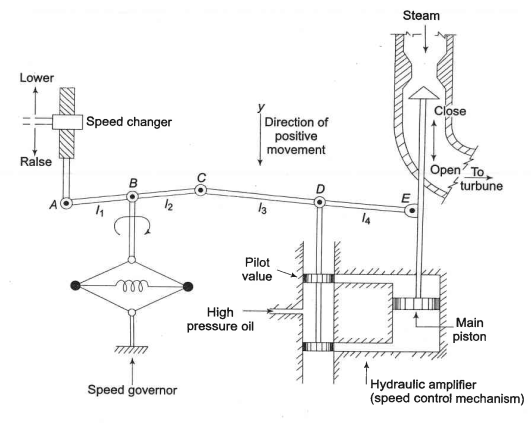
\includegraphics[scale=0.5]{A01_physical_governor_device}
	\caption{A schematic of a steam governor}
	\label{fig:A01_physical_governor_device}
\end{figure}

If we let $A$ on the in the schematic be moved downward a little bit, $\Delta y_A$, the turbine power output will change by a directly proportional amount. Letting $\Delta P_C$ be the power increase, this can be expressed as:
\begin{equation}
	\Delta y_A = k_C \Delta P_C \label{eq:A01}
\end{equation}

An increase in $\Delta P_C$ will cause the pilot valve to move up, and high pressure oil will flow onto the top of the main piston forcing it downwards. As the steam valve opens, more steam will drive the turbine faster and causing the flyball governor to lower point $B$. Mathematically, the movement of $C$ can be expressed as the result of two separate inputs:
\begin{enumerate}
	\item Assuming that $\Delta y_A$ is small, using similar triangles, it can be written that:
	\begin{equation}
    	\Delta y_C = - \frac{l_2}{l_1} \Delta y_A
	\end{equation}
	\item Given a frequency increase $\Delta f$ point $B$ will move downward so, assuming $A$ is fixed, then using similar triangles it is clear that:
	\begin{equation}
		\Delta y_C = \frac{l_1 + l_2}{l_1} \Delta y_B
	\end{equation}
\end{enumerate}

Letting $k_1 = \frac{l_2}{l_1}$, $k_2 = \frac{l_1 + l_2}{l_1} k_2'$, and using equation \ref{eq:A01}, the total movement in point $C$ can be expressed as:
\begin{equation}
	\Delta y_C = - k_1 k_C \Delta P_C + k_2 \Delta f \label{eq:A02}
\end{equation}

A similar analysis, considering movement of point $C$ and $E$, can be undertaken to mathematically express the movement of point $D$. The analysis also makes use of similar triangles and results in the expression:
\begin{equation}
	\Delta y_D = \frac{l_4}{l3 + l_4} \Delta y_C + \frac{l3}{l_3 + l_4} \Delta y_E
\end{equation}

Letting $k_3 = \frac{l_4}{l_3 + l_4}$ and $k_4 = \frac{l3}{l_3 + l_4}$, this can be re-expressed as:
\begin{equation}
	\Delta y_D = k_3 \Delta y_C + k_4 \Delta y_E \label{eq:A03}
\end{equation}

When there is some movement, $\Delta y_D$, of point $D$ the ports of the pilot valve will open and high pressure oil will plow onto the cylinder causing some movement $\Delta y_E$. If point $D$ moves up, high pressure oil will move point $E$ down, and conversely if point $D$ moves down, high pressure oil will move point $E$ upwards. To simplify the dynamics of this scenario, the following assumptions are made:
\begin{enumerate}
	\item Inertial reaction forces of the main piston and steam valve are negligible compared to the forces exerted on the piston by high pressure oil
	\item Due to the first assumption, the rate of oil admitted to to the cylinder is proportional to the port opening $\Delta y_D$.
\end{enumerate}

The volume of oil admitted to the cylinder is thus proportional to the time integral of $\Delta y_D$. Dividing the oil volume by the cross-sectional area of the piston:
\begin{equation}
	\Delta y_E = k_5 \int (- \Delta y_D) dt \label{eq:A04}
\end{equation}

Taking the Laplace transform of equations \ref{eq:A02}, \ref{eq:A03}, and \ref{eq:A04} gives the following:
\begin{align}
	\Delta Y_C(s) &= -k_1 k_C \Delta P_C(s) + k_2 \Delta F(s) \label{eq:A05} \\
	\Delta Y_D(s) &= k_3 \Delta Y_C(s) + k_4 \Delta Y_E(s) \label{eq:A06} \\
	\Delta Y_E(s) &= - k_5 \frac{1}{s} \Delta Y_D(s) \label{eq:A07}
\end{align}

Algebraically manipulating \ref{eq:A05}, \ref{eq:A06}, and \ref{eq:A07} eliminates $\Delta Y_C(s)$ and $\Delta Y_D(s)$ and results in the following equation:
\begin{equation}
	\Delta Y_E(s) = \frac{k_1 k_3 k_C \Delta P_C(s) - k_2 k_3 \Delta F(s)}{k_4 + \frac{s}{k_5}} \label{eq:A08}
\end{equation}

Equation \ref{eq:A08} can be re-expressed as:
\begin{equation}
	\Delta Y_E(s) = \bigg[ \Delta P_C(s) - \frac{1}{R} \Delta F(s) \bigg] \times \bigg( \frac{K_{sg}}{1 + T_{sg}s} \bigg) \label{eq:A09}
\end{equation}

where
\begin{align}
	R &= \frac{k_1 k_C}{k_2} \\
	K_{sg} &= \frac{k_1 k_3 k_C}{k_4} \\
	T_{sg} &= \frac{1}{T_{sg}} 
\end{align}

Equation \ref{eq:A09} is the model of the governor in the frequency domain. The parameter $R$ is referred to as the speed regulation of the governor; the parameter $K_{sg}$ is referred to as the gain of the speed governor; and the parameter $T_{sg}$ is referred to as the time constant of the speed governor.

The complete block diagram of governor model can be seen in Figure \ref{fig:A02_governor_model} below.

\begin{figure}[h]
	\centering
	\begin{tikzpicture}

\end{tikzpicture}
	\caption{Block diagram of the steam governor model in the frequency domain}
	\label{fig:A02_governor_model}
\end{figure}